\documentclass{article}
\usepackage[utf8]{inputenc}
\usepackage[legalpaper, portrait, margin=0.5in]{geometry}
\usepackage[spanish,es-tabla]{babel}

\title{Trabajo Práctico 1: Conceptos básicos}
\author{Emmanuel Ferreyra, Bruno Kaufman, Ariel Salgado}
\date{\today}

\usepackage{natbib}
\usepackage{graphicx}

\begin{document}

\maketitle

\section{Problema 1}
En este punto se pide analizar tres redes complejas de interacción de proteinas. La primera se trata de interacciones binarias entre proteinas, la segunda de co-pertenencia a complejos, y la tercera una obtenida del proyecto Yeast Interactome Database (YID).

Las tres redes se visualizan en la tabla \ref{comparacionvisualP1}.
%% Fijate de incluir una mención a cada red en el texto, que no esté solo en la figura. Y también poner las redes "completas", no cortadas en dos.
\begin{table}[ht]
\caption{\textbf{Superior:} Componente gigante perteneciente a la red de interacciones binarias (APMS), de co-pertenencia (LIY), y del proyecto YID (Y2H), de izquierda a derecha. \textbf{Inferior:} misma información respecto a las componentes pequeñas de las redes.}
\centering
\begin{tabular}{ccc}
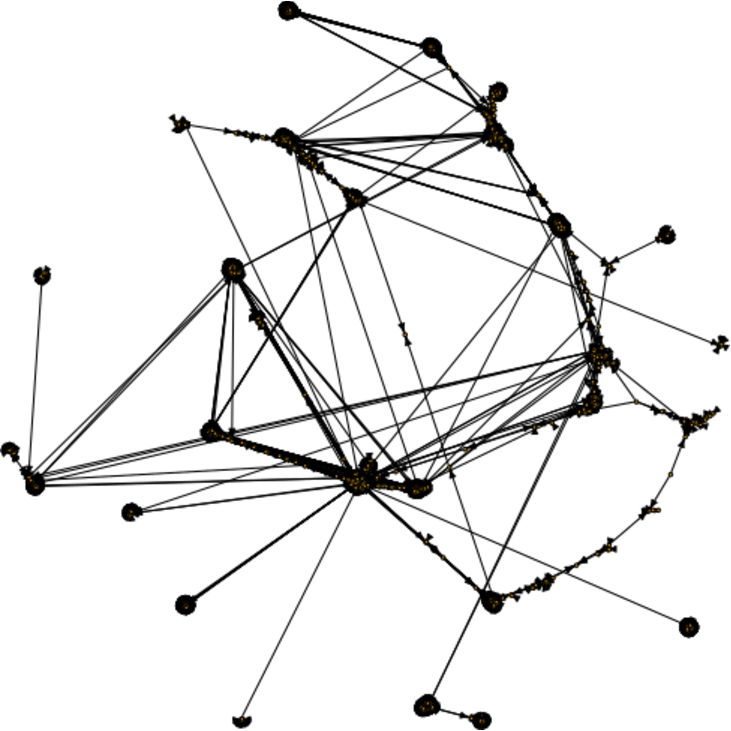
\includegraphics[scale=0.4]{Imagenes_P1/APMSgigante.pdf}&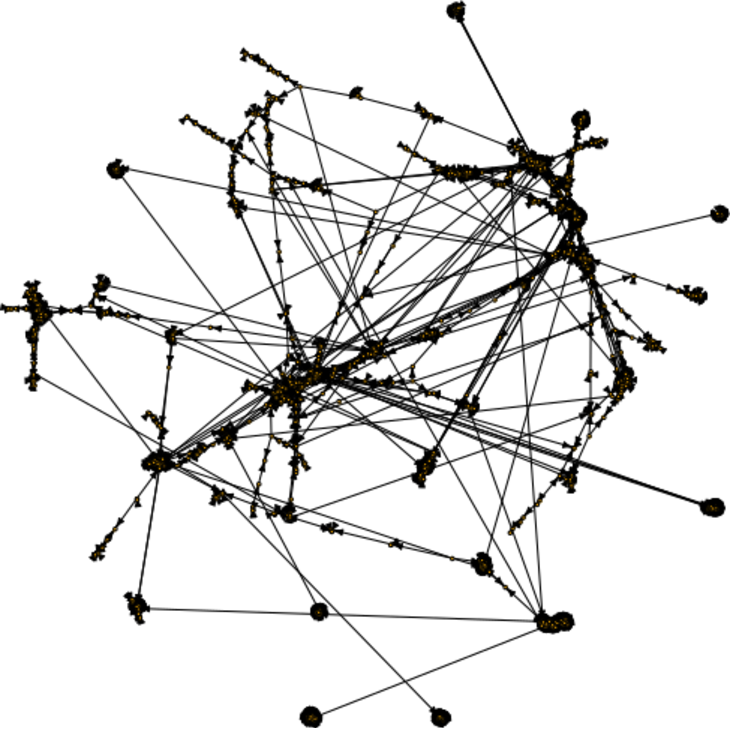
\includegraphics[scale=0.4]{Imagenes_P1/LITgigante.pdf}&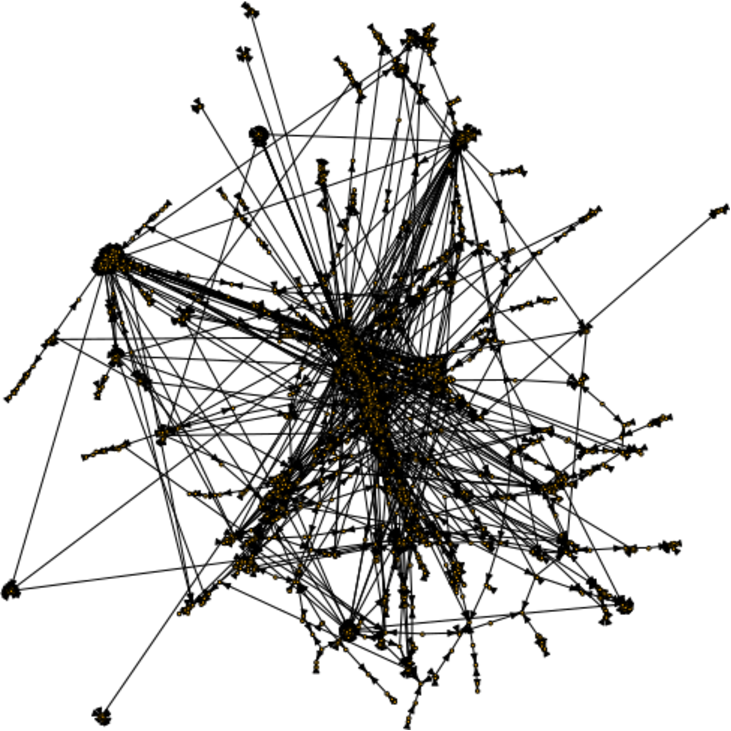
\includegraphics[scale=0.4]{Imagenes_P1/Y2Hgigante.pdf}\\
 
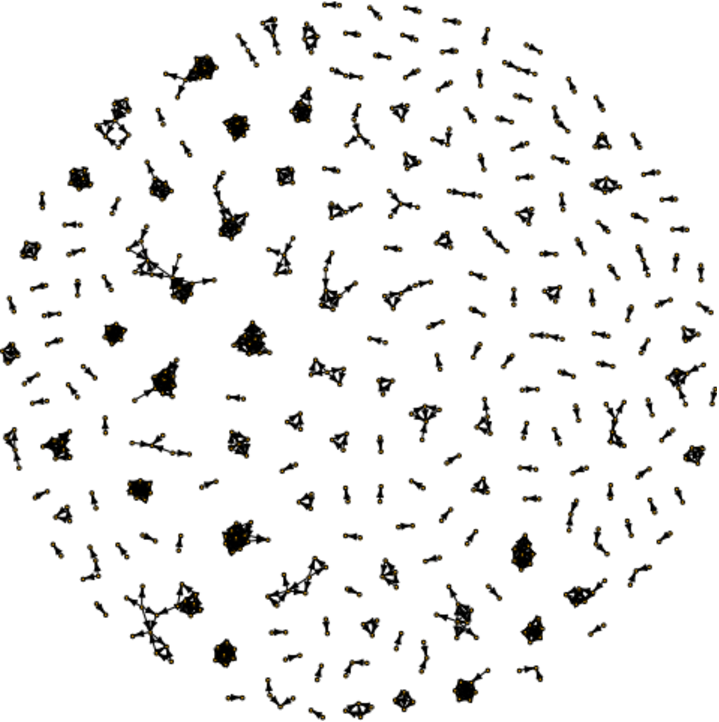
\includegraphics[scale=0.4]{Imagenes_P1/APMSchiquitos.pdf}&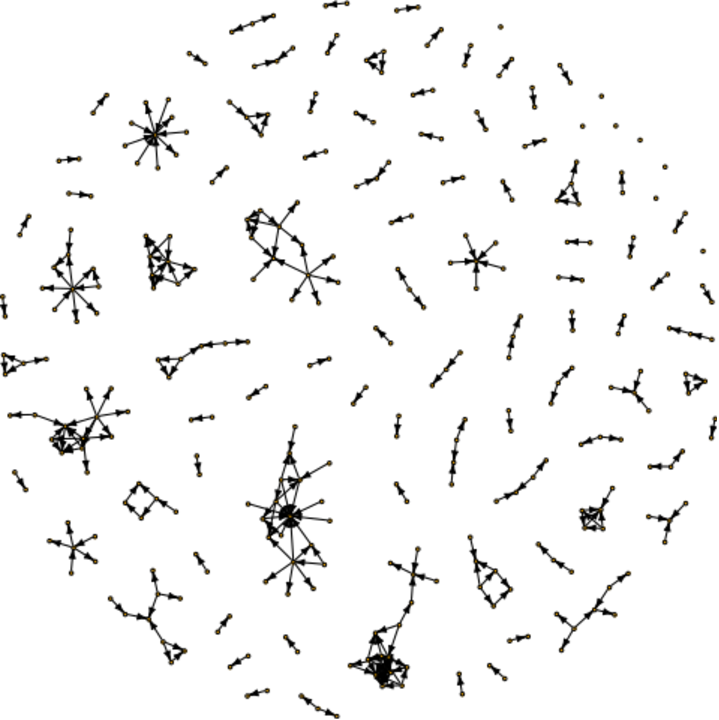
\includegraphics[scale=0.4]{Imagenes_P1/LITchiquitos.pdf}&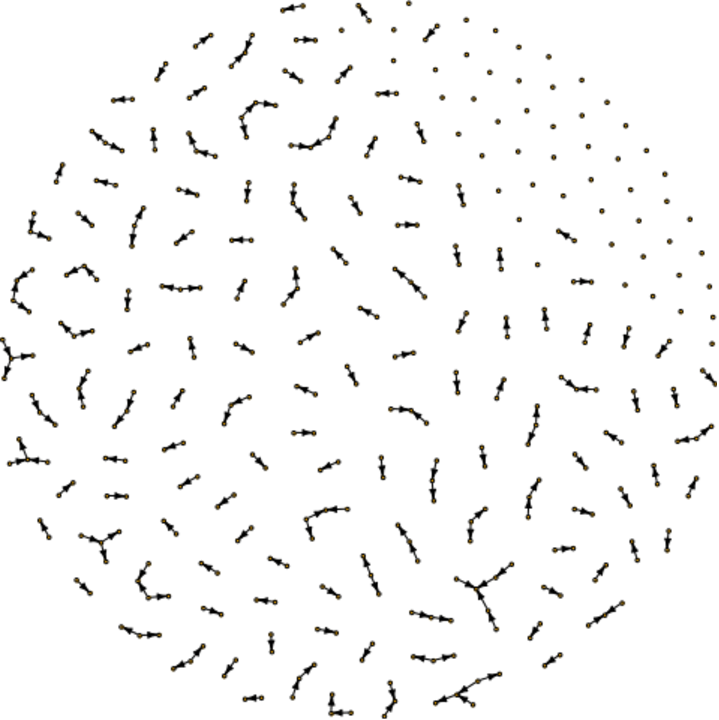
\includegraphics[scale=0.4]{Imagenes_P1/Y2Hchiquitos.pdf}\\
\end{tabular}
\label{comparacionvisualP1}
\end{table}


\section{Problema 2}
En el segundo problema se propone analizar una red social de 62 delfines de Nueva Zelanda. La red consta de 34 machos, 24 hembras y 4 delfines de sexo desconocido. La base de datos establece 159 vinculos entre los delfines de la red.

\subsection{Punto 2.a.}
El primer objetivo es comparar diferentes opciones de layout para graficar la red, comparando ventajas y desventajas. Para esto empleamos el paquete \texttt{igraph} de \texttt{R}. El mismo provee distintas opciones de layout a partir de funciones predeterminadas. Presentamos para ejemplificar tres layouts: \texttt{layout-with-fr},\texttt{layout-as-tree} y \texttt{layout-on-grid}. El primero construye el layout a partir de un cálculo de equilibrio de fuerzas, el segundo intenta representar al grafo como un árbol, permitiendo que se le indique un nodo semilla, y el tercero posiciona los nodos sobre una grilla regular. En la figuras \ref{pt2layouts} se pueden observar los mismos. Los nodos rojos representan los machos, los azules las hembras, y los negros los de sexo desconocido. Ninguno de los últimos dos facilita la visualización del gráfico, indicando que las estructuras propuestas no son representativas de la estructura del grafo. Por otro lado, \texttt{layout\_with\_fr}, al tener directamente en cuenta los vinculos de la red para su construcción, nos permite observar que hay dos grupos de delfines bastante diferenciados, uno en el que predominan las hembras (y dominan los colores azules) y otro donde predominan los machos (mayoría de colores rojos).

\begin{figure}[!htb]
   \begin{minipage}{0.3\textwidth}
	\centering
	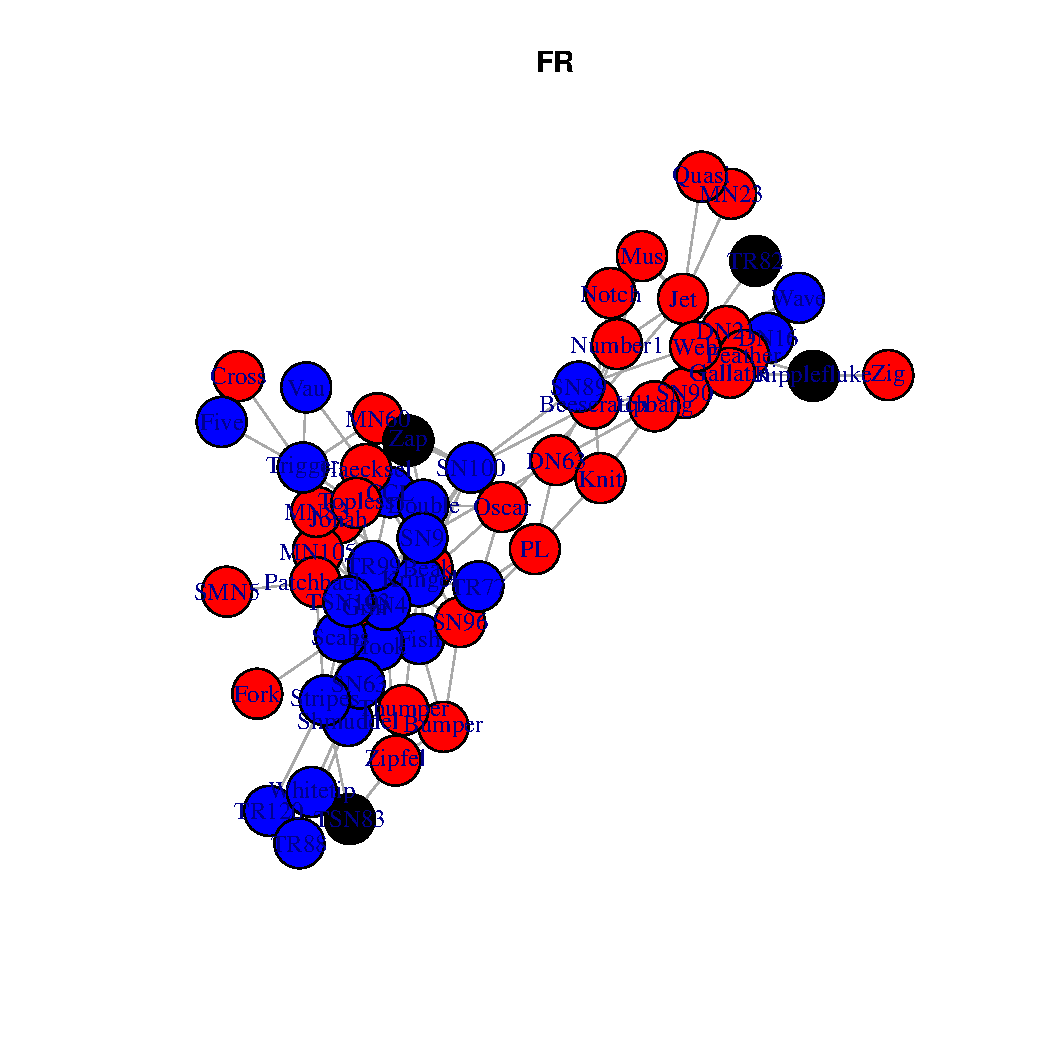
\includegraphics[width=.7\linewidth]{Imagenes_P1/layout_dolphins2.pdf}
%	\caption{Red de los delfines, graficada según \textt{layout\_with\_fr}.}
	\label{pt2layoutsfr}
   \end{minipage}\hfill
   \begin{minipage}{0.3\textwidth}
	\centering
	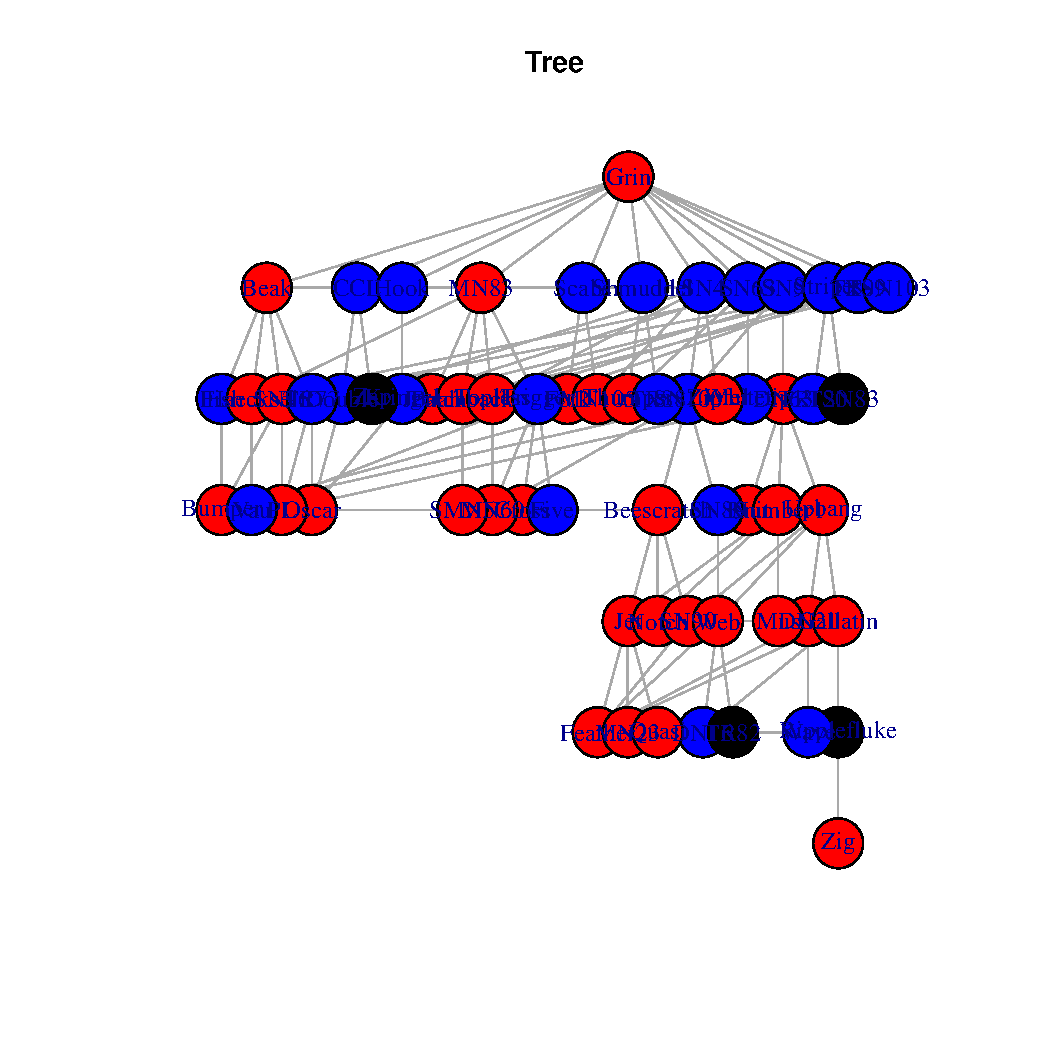
\includegraphics[width=.7\linewidth]{Imagenes_P1/layout_dolphins3.pdf}
%	\caption{Red de los delfines, graficada seg\'un \textt{layout\_as\_tree}.}
	\label{pt2layouttree}
   \end{minipage}\hfill
   \begin{minipage}{0.3\textwidth}
	\centering
	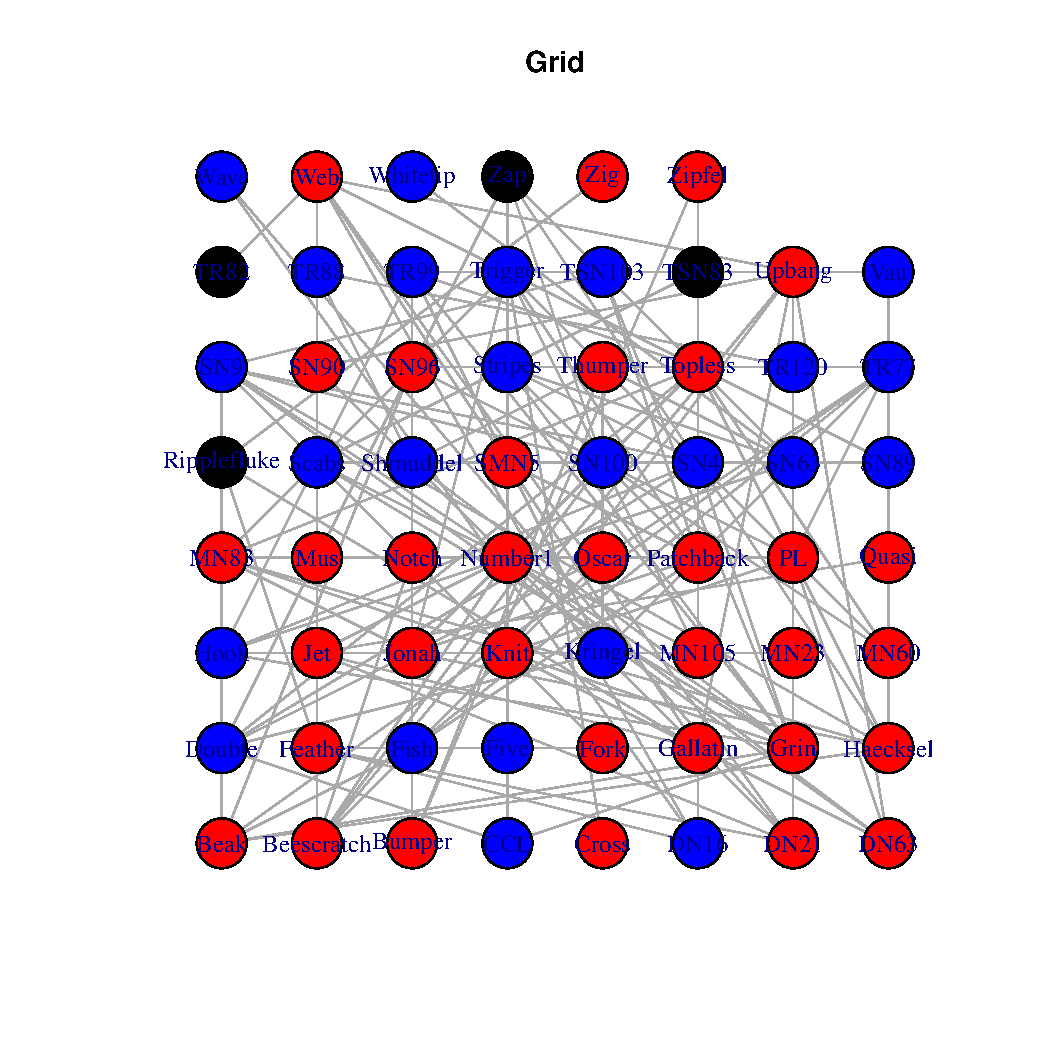
\includegraphics[width=.7\linewidth]{Imagenes_P1/layout_dolphins7.pdf}
%	\caption{Red de los delfines, graficada seg\'un \textt{layout\_on\_grid}.}
	\label{pt2layoutgrid}
   \end{minipage}
   \label{pt2layouts}
\end{figure}


\subsection{Punto 2.b.}
En este punto se propone testear la hipótesis que sugiere \texttt{layout\_with\_fr}: que hay más vinculos entre delfines del mismo sexo (vinculos homofilos) que entre delfines de distinto sexo (vinculos heter\'ofilos). Para esto, calculamos la fracción de ejes que conectan delfines de distinto sexo como

\begin{equation}
    f_{mf} = \frac{1}{M}\sum_{ij} A_{ij} \delta_{s_i,m} \delta_{s_j,f}
\end{equation}

donde $s_i$ es el sexo del delfin $i$ y $A_{ij}$ es la matriz de adyacencia del red, y $M = \sum_{ij} A_{ij}/2$ es la cantidad de ejes en la red. De forma análoga, calculamos las fracciones de ejes que conectan hembras con hembras y machos con machos:

\begin{equation}
        f_{m} = \frac{1}{2M}\sum_{ij} A_{ij} \delta_{s_i,m} \delta_{s_j,m} 
\end{equation}
\begin{equation}
        f_{f} = \frac{1}{2M}\sum_{ij} A_{ij} \delta_{s_i,f} \delta_{s_j,f} 
\end{equation}
En todos los casos, consideramos únicamente los defines con sexo conocido. Obtenemos los valores de $f_{mf} = 0.327$, $f_{m} = 0.377$ y $f_{f} = 0.226$, quedando aproximadamente un $7\%$ de los ejes sin considerar por no conocerse el sexo. Para saber si estos valores son altos o bajos, el ejercicio propone reasignar de forma azarosa los sexos de cada delfín, y calcular las tres fracciones para cada asignación de sexo. Realizando 1000 reasignaciones, obtenemos tres distribuciones de valores. Podemos observar estos en la figura \ref{pt2histogramas}. Obtenemos valores esperados de $\widehat{f_{mf}} = 0.43 \pm 0.04$, $\widehat{f_{m}} = 0.30 \pm 0.04$ y $\widehat{f_{f}} = 0.15 \pm 0.03$, de donde vemos que los valores observados se encuentran entre 1.8 y 2.8 sigmas de distancia de los esperados. Si calculamos los $p$ valores en cada caso, obtenemos $p_{mf} = 0.005$,$p_m = 0.029$ y $p_f = 0.015$, indicando una muy baja probabilidad de que por azar la estructura observada se forme.

\begin{figure}[!htb]
   \begin{minipage}{0.3\textwidth}
	\centering
	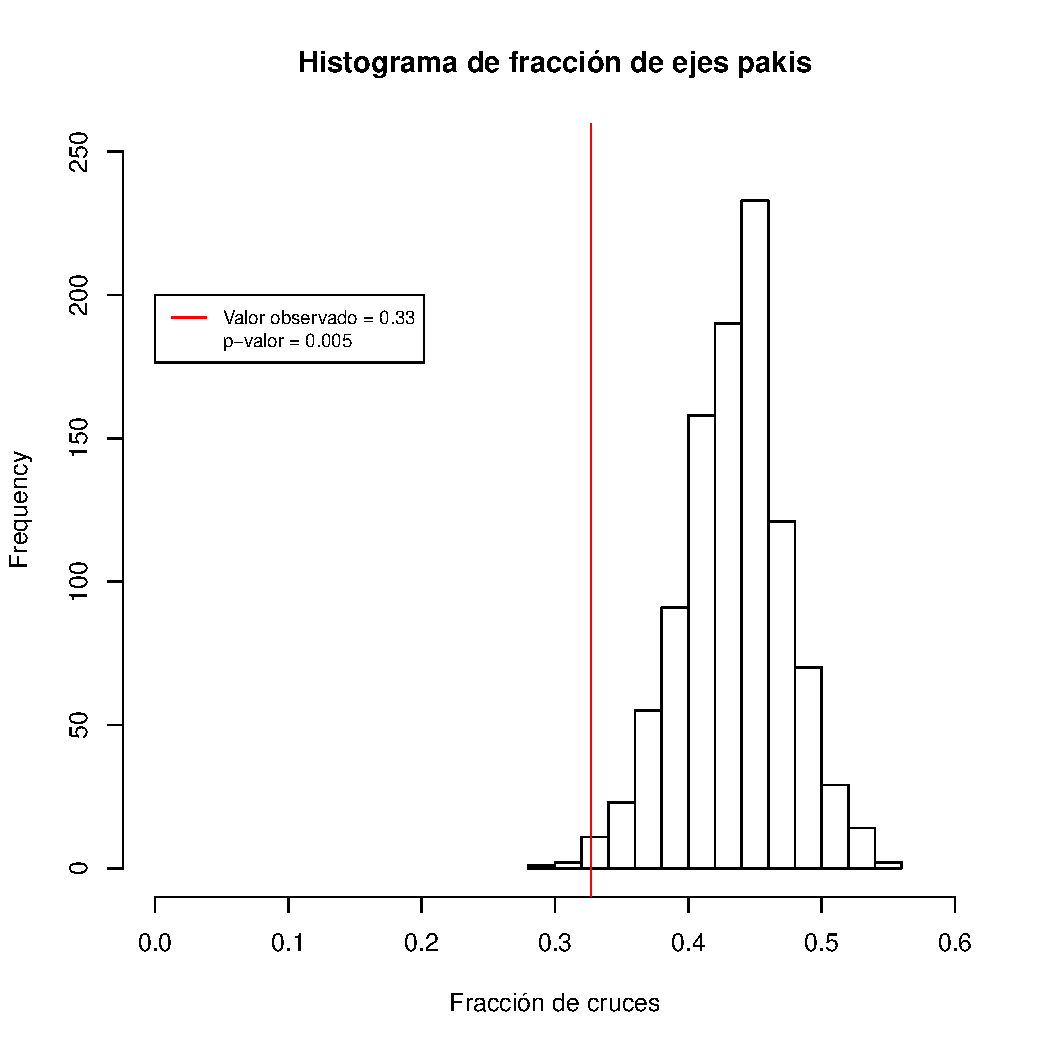
\includegraphics[width=.7\linewidth]{Imagenes_P1/histo_homofilia1.pdf}
	\caption{Histograma de fracción de ejes que conectan delfines de sexos distintos.}
	\label{pt2histo-cruces}
   \end{minipage}\hfill
   \begin{minipage}{0.3\textwidth}
	\centering
	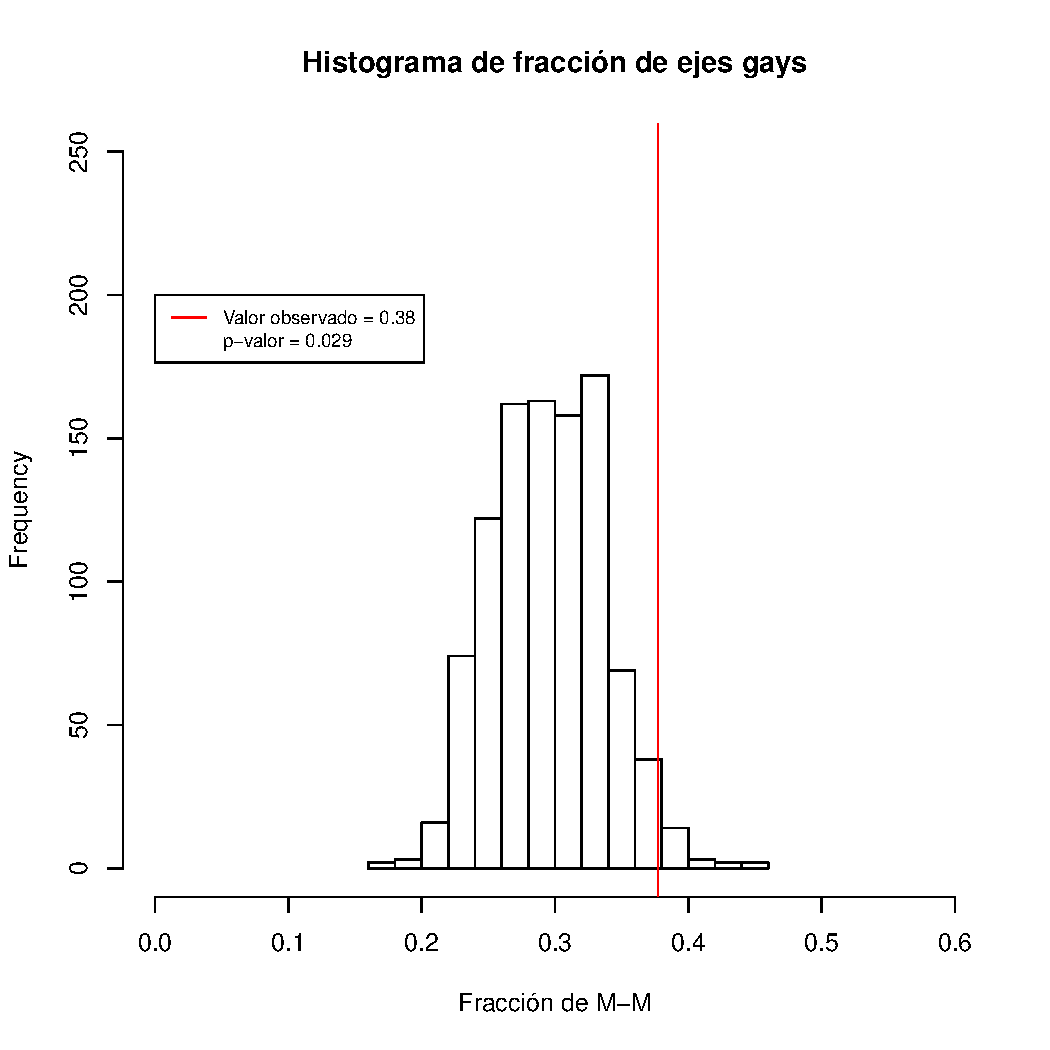
\includegraphics[width=.7\linewidth]{Imagenes_P1/histo_homofilia2.pdf}
	\caption{Histograma de fracción de ejes que conectan defines macho con macho.}
	\label{pt2histo-mym}
   \end{minipage}\hfill
   \begin{minipage}{0.3\textwidth}
	\centering
	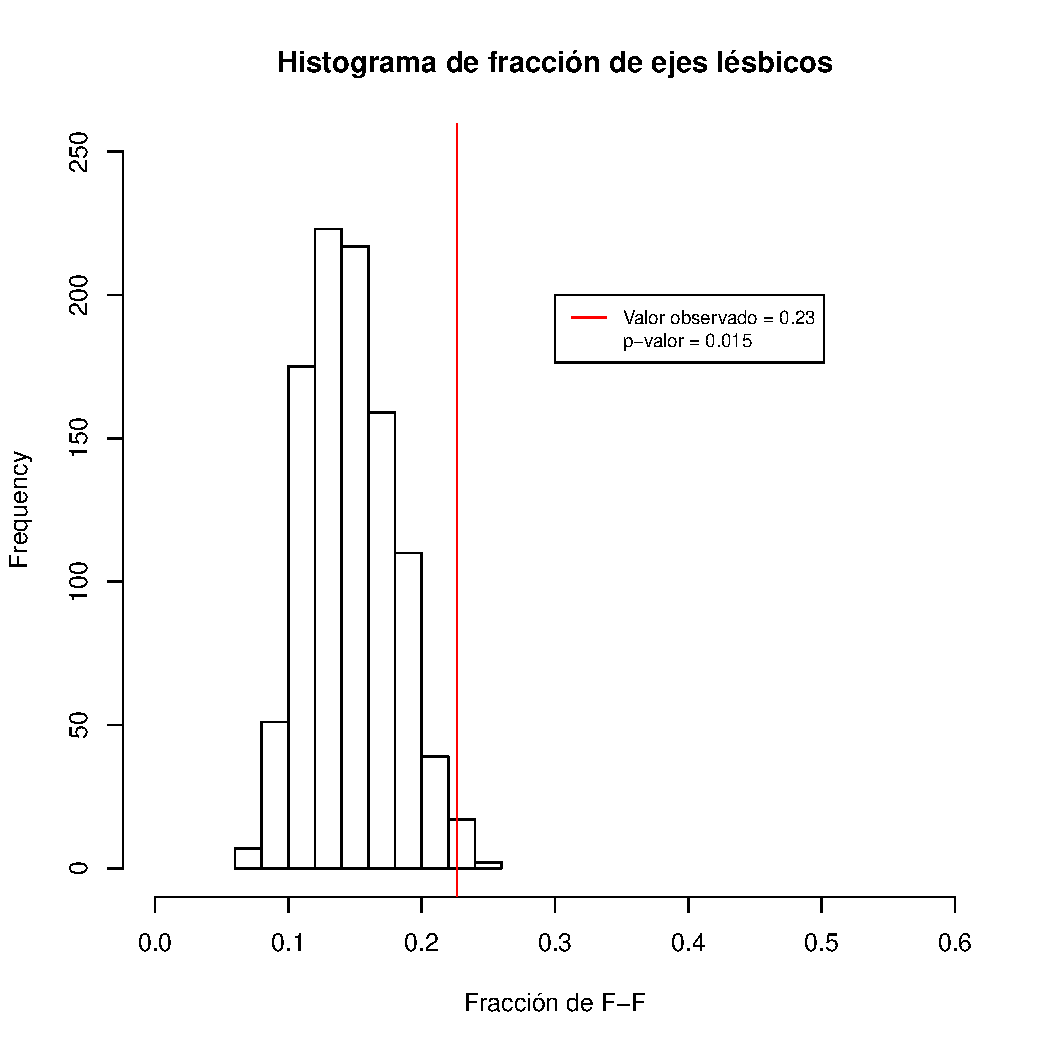
\includegraphics[width=.7\linewidth]{Imagenes_P1/histo_homofilia3.pdf}
	\caption{Histograma de fracción de ejes que conectan defines hembra con hembra.}
	\label{pt2histo-fyf}
   \end{minipage}
   \label{pt2layout}
\end{figure}

\subsection{Punto 2.c.}
Por último, el ejercicio propone comparar distintas estrategias para remover nodos de la red, basandose en la estructura de la misma. Para esto proponemos 4 estrategias: extraer nodos según su grado, su coeficiente local de clustering, su betwenness (una medida de la cantidad de caminos mínimos que atraviezan un eje) y extraer completamente al azar. En la figura \ref{rupturas} podemos observar el tamaño de la primer y segunda componente. Elegimos la estrategia más apropiada viendo cual asemeja los tamaños más prontamente. Vemos que la estrategia más exitosa es la que extrae por betweenness. Seguida de ella está extraer por grado, que tiene éxito cuando las componentes ya son más pequeñas. Por último, extraer según el coeficiente de clustering no da un resultado muy distinto del azar.

\section{Problema 3}
En este ejercicio estudiamos la distribución de grados $P_k$ como función de $k$. Nuevamente utilizamos las funciones del paquete \texttt{igraph} de \texttt{R}, consiguiendo primero los grados de cada nodo y luego utilizando el comando \texttt{hist} 	que computa un histograma a partir del vector de grados.

En la siguiente tabla están los gráficos con distintas alternativas, con bineado lineal o logarítmico y utilizando diferentes escalas.

\begin{figure}[!htb]
   \begin{minipage}{0.3\textwidth}
	\centering
	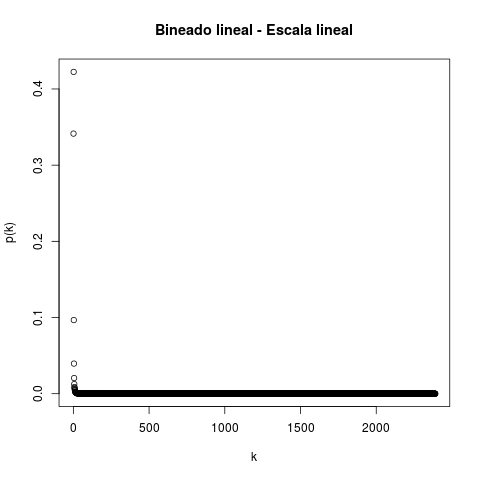
\includegraphics[width=.7\linewidth]{Imagenes_P3/P3_binlin_lin.png}
	\caption{Bineado Lineal - Escala lineal}
	\label{pt3linlinlin}
   \end{minipage}\hfill
   \begin{minipage}{0.3\textwidth}
	\centering
	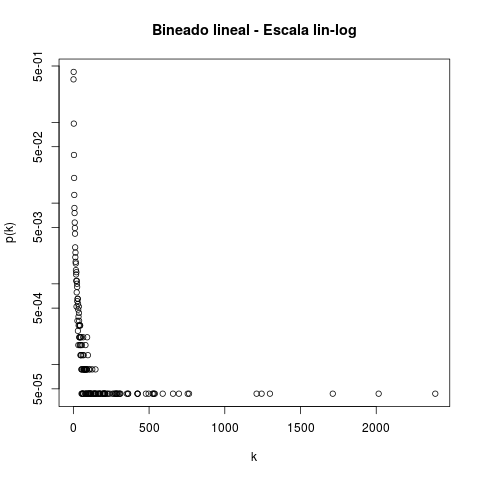
\includegraphics[width=.7\linewidth]{Imagenes_P3/P3_binlin_linlog.png}
	\caption{Bineado Lineal - Escala lineal en x logarítmica en y}
	\label{pt3linlinlog}
   \end{minipage}\hfill
   \begin{minipage}{0.3\textwidth}
	\centering
	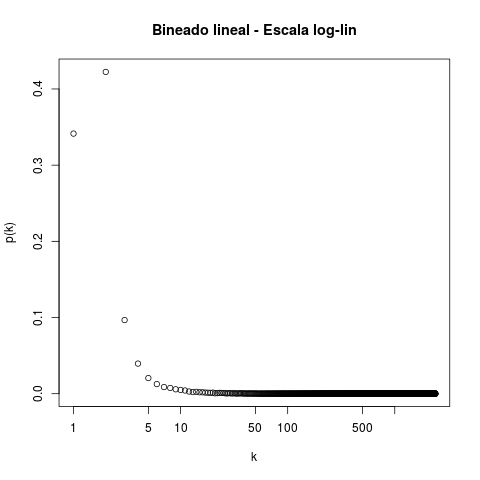
\includegraphics[width=.7\linewidth]{Imagenes_P3/P3_binlin_loglin.png}
	\caption{Bineado Lineal - Escala logarítmica en x lineal en y}
	\label{pt3linloglin}
   \end{minipage}\hfill
      \begin{minipage}{0.3\textwidth}
	\centering
	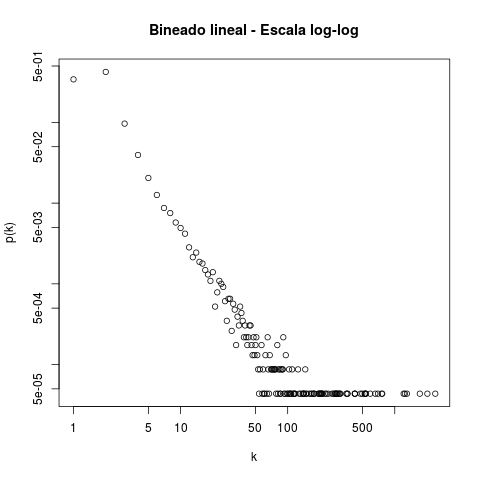
\includegraphics[width=.7\linewidth]{Imagenes_P3/P3_binlin_loglog.png}
	\caption{Bineado Lineal - Escala logarítmica}
	\label{pt3linloglog}
   \end{minipage}\hfill
      \begin{minipage}{0.3\textwidth}
	\centering
	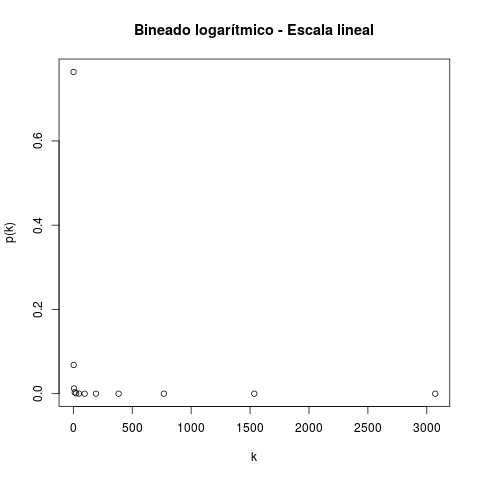
\includegraphics[width=.7\linewidth]{Imagenes_P3/P3_binlog_lin.png}
	\caption{Bineado logarítmico - Escala lineal}
	\label{pt3loglin}
   \end{minipage}\hfill
      \begin{minipage}{0.3\textwidth}
	\centering
	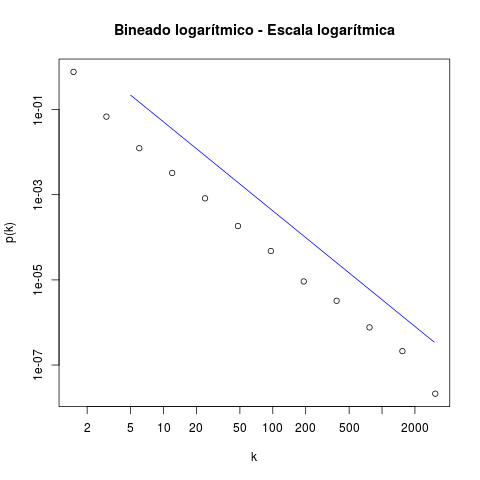
\includegraphics[width=.7\linewidth]{Imagenes_P3/P3_binlog_log.png}
	\caption{Bineado logarítmico - Escala logarítmica - Con recta del ajuste PL}	
	\label{pt3loglog}
   \end{minipage}\hfill
   \label{pt2layout}
\end{figure}

En las figuras 4 a 6 podemos ver la distribución de grados utilizando un bineado lineal. Se se aprecia la forma de la distribución aunque es complicado cuantificar si un ajuste libre de escala será coherente. En figuras \ref{pt3loglin} y \ref{pt3loglog} se utilizó un bineado logarítmico en base 2, y en la escala logarítmica se aprecia bien el carácter libre de escala de dicha distribución.

En la figura \ref{pt3loglog} se agregó la recta de ajuste libre de escala obtenida vía el comando \textit{fit\_power\_law} utilizando una malla de $3000$ puntos a partir del $k_{min}$ que en nuestro caso toma valor $5$. El valor estimado es $\alpha=2.097157$ ajustandose correctamente aunque corrido hacia arriba. Esto se debe a que el parámetro de normalización, es decir, la ordenada al origen, se calcula teniendo en cuenta todos los valores de grado, no solo los mayores al $k_{min}$.



\bibliographystyle{plain}
\bibliography{references}
\end{document}
